\documentclass[12pt,twoside]{book}
\usepackage{../../thesis}
\graphicspath{ {../../images/} }

\begin{document}

\chapter{Introduction}
In this chapter, I will introduce the logistic map as an example of a chaotic system.
Also, I will discuss the origin of chaos.

\section{Our First Chaotic Map}
This is the equation for logistic map:
\begin{equation}
  L_{\mu}(x) = \mu x(1-x),
  \label{logistic}
\end{equation}
and the ``equivalent'' differential equation:
\begin{equation}
  \frac{dx}{dt} = \mu x(1-x)
  \label{logisticdiffeq}
\end{equation}
(In general, we can go between continuous and discrete models
\begin{align*}
  \frac{dx(t)}{dt} = G(x(t)) &\quad\mbox{(Continuous)} \\
  x(t + 1) = F(x(t)) &\quad\mbox{(Discrete)}
\end{align*}
by using the following approximation of the differential equation by mapping
\begin{equation*}
  \frac{dx(t)}{dt} \approx \frac{x(t_0 + (n+1)\Delta t) - x(t_0 + n \Delta t)}{\Delta t},
\end{equation*}
which leads to an approximation of the mapping by the differential equation
\begin{equation*}
  F(x(n)) \approx x(n) + \Delta t \cdot G(x(n))
\end{equation*}
.)
The only difference between equations \pref{logisticdiffeq} and \pref{logistic}

The differential equation \pref{logisticdiffeq} can be easily solved by separation of variables.
\begin{align*}
  \frac{dx}{x(1-x)} &= \mu dt \\  
  \left( \frac{1}{x} + \frac{1}{1-x} \right) dx &= \mu dt
\end{align*}
Then, suppose that $x(0) = x_0$, and integrate from $t = 0$ to $T$
\begin{align*}
  \int_{x_0}^{x(T)} \frac{1}{x} + \frac{1}{1-x} dx &= \int_0^T \mu dt \\
  \log{\frac{x(T)}{1-x(T)}} - \log{\frac{x_0}{1-x_0}} &= \mu T \\
  \frac{x(T)}{1-x(T)} &= \frac{x_0 e^{\mu T}}{1-x_0} \\
  (1-x_0)x(T) &= x_0 e^{\mu T} (1-x(T)) \\
  (1-x_0 + x_0 e^{\mu T})x(T) &= x_0 e^{\mu T}
\end{align*}

Thus, we have (with a slight change of notation)
\begin{equation}
  x(t) = \frac{x_0 e^{\mu t}}{1 - x_0 + x_0 e^{\mu t}}
  \label{eq:logisticdiffeqsoln}
\end{equation}

Change in the growth rate $\mu$ does not alter the bahaviour.
\begin{figure}[ht]
  \begin{center}
    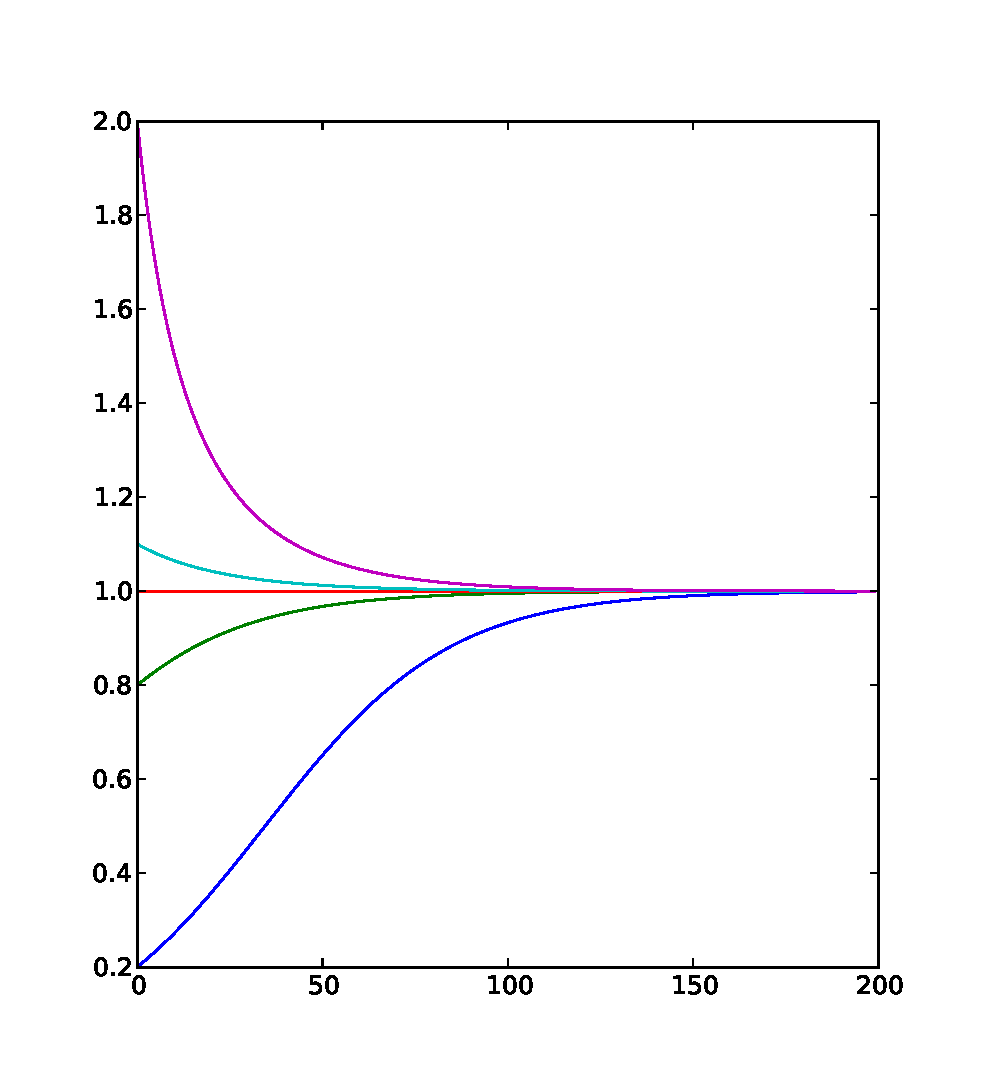
\includegraphics[scale=0.5]{logistic_diffeq_mu4_varyingx0}
  \end{center}
  \caption{
    Plot of equation \pref{eq:logisticdiffeqsoln} with $\mu = 4$ and various $x_0$. 
  Note that regardless of the initial value, $x(t)$ converges to $1$.
}
  \label{fig:logistic_diffeq1}
\end{figure}

%\begin{figure}[h]
%  \begin{center}
%    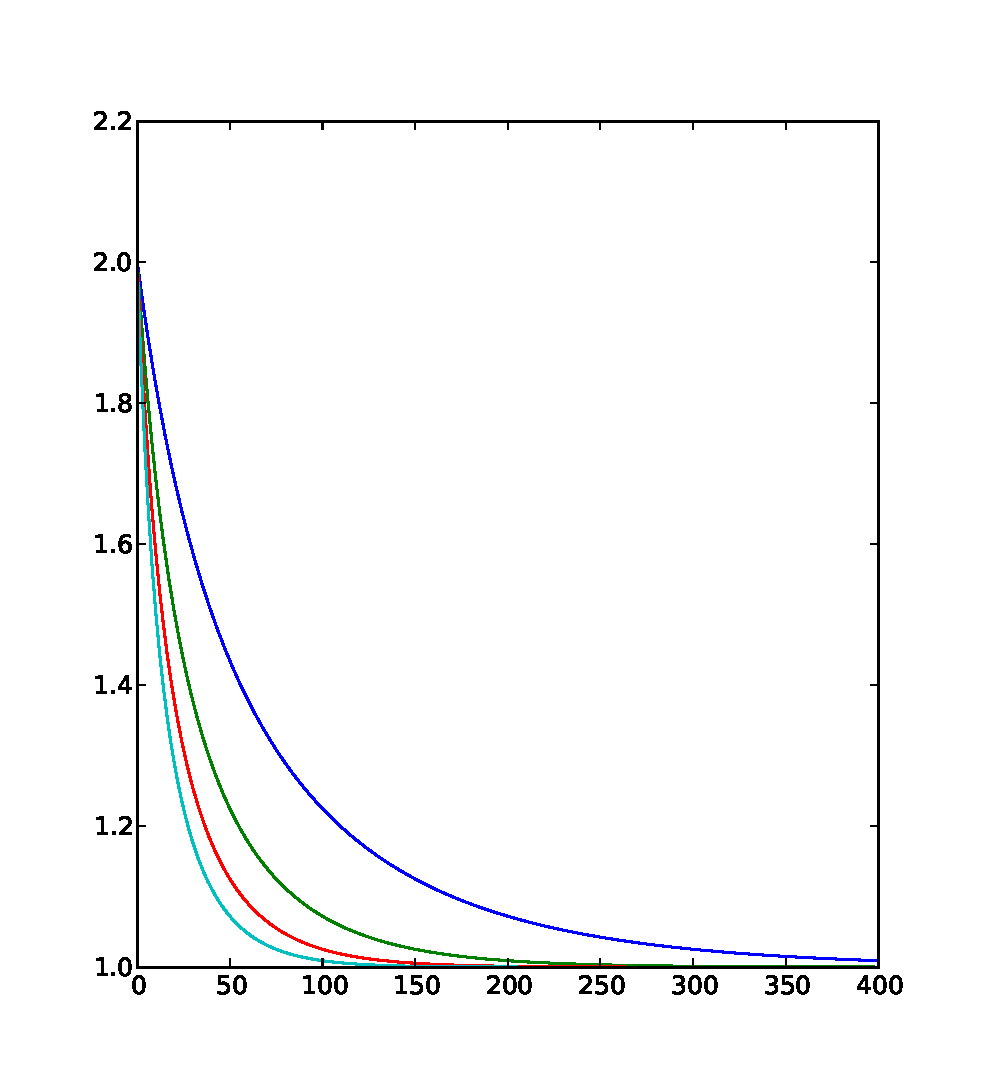
\includegraphics[scale=0.5]{logistic_diffeq_mu1234_x2}
%  \end{center}
%  \caption{
%    Plot of equation \pref{eq:logisticdiffeqsoln} with $x_0 = 2$ and various $\mu$ (1,2,3,4).
%    As $\mu$ increases, $x(t)$ converges to $1$ faster.
%    However, it does not alter the overall behaviour.
%  }
%  \label{fig:logistic_diffeq2}
%\end{figure}

\begin{figure}[h]
  \begin{center}
    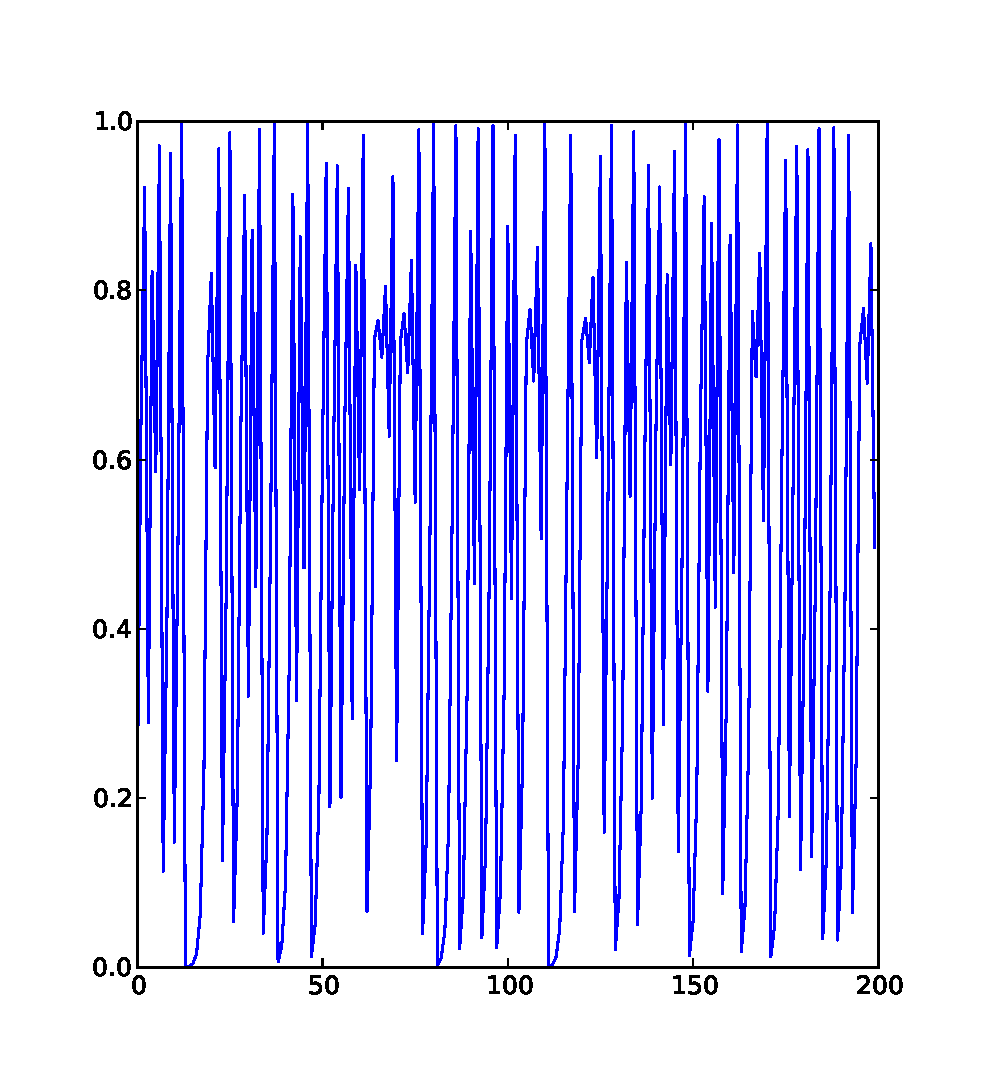
\includegraphics[scale=0.5]{logistic_map_mu4_x02}
  \end{center}
  \caption{
    Chaotic map.
  }
  \label{fig:logistic_map_chaotic}
\end{figure}

\section{The Origin of Chaos}
Edward Lorentz is commonly known as the first discoverer of chaos.
\begin{figure}[t]
  \begin{center}
    \includegraphics[scale=0.5]{golden_lorentz_attractor}
  \end{center}
  \caption{Lorentz Attractor}
  \label{fig:lorentz}
\end{figure}
He found chaotic behaviours through atmospheric simulations using twelve differential equations.
In his seminal article ``Deterministic Nonperiodic Flow'', Lorentz discusses the chaotic behavior of three differential equations, which were reduced from the original twelve equations.
However, I would like to introduce Yoshisuke Ueda, who, though lesser known, was the first scientist to notice chaos in 1961 (a sketch of the ``Japanese Attractor''), while Lorentz's paper was published in 1963.
David Ruelle, a prominent French chaos researcher, introduced Ueda in 1978 (in Thermodynamic Formalism?).
\footnote{Doubtful of Ueda's result, Ueda's mentor did not allow publication of Ueda's result until 1970, seven years after the publication of ``Deterministic Nonperiodic Flow.''
Because of the strict hierarchical structure of the Japanese academia, the first author of Ueda's paper, ``On the Behavior of Self-Oscillatory Systems with External Force'', is his mentor.%\cite[p89]{sprott}
% 君が見たのは単に概周期振動にすぎない。概念的な所見を述べるのは、若い君のやることじゃない。
He left the following remark: ``Chaos, though common phenomena in the nature, has been dismissed because of the difficulty to grasp its full notion.''\citep[p533]{gleick}
Either way, vigorous research activities on chaos only started in the 70's.}
The reason that I would like to discuss this scientist instead of Lorentz is not because he is the first scientist to see chaos.
The name ``Japanese Attractor'' was given by David Ruelle.
% Ueda: 最初はアナログコンピュータが故障したのかと思った。しかしすぐに、いやそんなことはないと悟った (in Chaos Avant-Garde?)
``I thought vaccum tubes were broken or something---a common issues with computers of those days.'' \citep{lorentzbook} %私はすぐに真空管が弱ったか何かの、よくあるコンピュータトラブルを疑ったが、修理を頼む前に、どこで間違いが起ったかだけでも調べてみることにした
%「カオス現象は、われわれが、日常、目にしているありふれた実在の自然現象であるにもかかわらず、その概念把握の困難さのために、かっては見過ごされてきた」
The true value in Ueda's findings lies in its settings.
While Lorentz's discovery of chaos was through computer simulation of a hypothetical model, Ueda's was through a physical, real-world system.
The first experimental confirmation of chaos was due to Liebacher using Helium.

\section{So What Is Chaos, After All?}
We tend to label a dynamical systems as ``chaotic'' on an intuitive ground.
If the orbit looks (judged by our visual sense organ complex), the system is called chaotic.
In 1986, the Royal Society held an international conference on chaos and defined ``chaos'' as ``Stochastic behavior occurring in a deterministic system.'' \cite{stewart}
Two Russian physicists famously said "A strange attractor seems strange only to a stranger."
(Boris Chirikov, Felix Izrailev)\cite{lorentzbook}

\bibliographystyle{../../bibliography/pjgsm}
\bibliography{../../bibliography/thesis}
\end{document}
